%-------------------------
% Resume in Latex
% Author : Sourabh Bajaj
% License : MIT
%------------------------

\documentclass[letterpaper,11pt]{article}

\usepackage{CJKutf8}
\usepackage{graphicx}
\usepackage{latexsym}
\usepackage[empty]{fullpage}
\usepackage{titlesec}
\usepackage{marvosym}
\usepackage[usenames,dvipsnames]{color}
\usepackage{verbatim}
\usepackage{enumitem}
\usepackage[hidelinks]{hyperref}
\usepackage{fancyhdr}
\usepackage[english]{babel}
\usepackage{tabularx}

\pagestyle{fancy}
\fancyhf{} % clear all header and footer fields
\fancyfoot{}
\renewcommand{\headrulewidth}{0pt}
\renewcommand{\footrulewidth}{0pt}

% Adjust margins
\addtolength{\oddsidemargin}{-0.5in}
\addtolength{\evensidemargin}{-0.5in}
\addtolength{\textwidth}{1in}
\addtolength{\topmargin}{-.5in}
\addtolength{\textheight}{1.0in}

\urlstyle{same}

\raggedbottom
\raggedright
\setlength{\tabcolsep}{0in}

% Sections formatting
\titleformat{\section}{
  \vspace{-4pt}\scshape\raggedright\large
}{}{0em}{}[\color{black}\titlerule \vspace{-5pt}]

%-------------------------
% Custom commands
\newcommand{\resumeItem}[2]{
  \item\small{
    \textbf{#1}{: #2 \vspace{-2pt}}
  }
}

\newcommand{\resumeSubheading}[4]{
  \vspace{-1pt}\item
    \begin{tabular*}{0.97\textwidth}[t]{l@{\extracolsep{\fill}}r}
      \textbf{#1} & #2 \\
      \small #3 & \small #4 \\
    \end{tabular*}\vspace{-5pt}
}

\newcommand{\resumeSubItem}[2]{\resumeItem{#1}{#2}\vspace{-4pt}}

\renewcommand{\labelitemii}{$\circ$}

\newcommand{\resumeSubHeadingListStart}{\begin{itemize}[leftmargin=*]}
\newcommand{\resumeSubHeadingListEnd}{\end{itemize}}
\newcommand{\resumeItemListStart}{\begin{itemize}}
\newcommand{\resumeItemListEnd}{\end{itemize}\vspace{-5pt}}

%-------------------------------------------
%%%%%%  CV STARTS HERE  %%%%%%%%%%%%%%%%%%%%


\begin{document}

%----------HEADING-----------------
\begin{tabular*}{\textwidth}{l@{\extracolsep{\fill}}r}
  \textbf{\href{https://www.fosskers.ca/}{\Large Colin Woodbury}} & Email : \href{mailto:colin@fosskers.ca}{colin@fosskers.ca}\\
  \href{https://www.fosskers.ca/jp/cv}{https://www.fosskers.ca/jp/cv} & Mobile : +1-604-812-4532 \\
\end{tabular*}

\begin{figure}[h!]
  \centering
  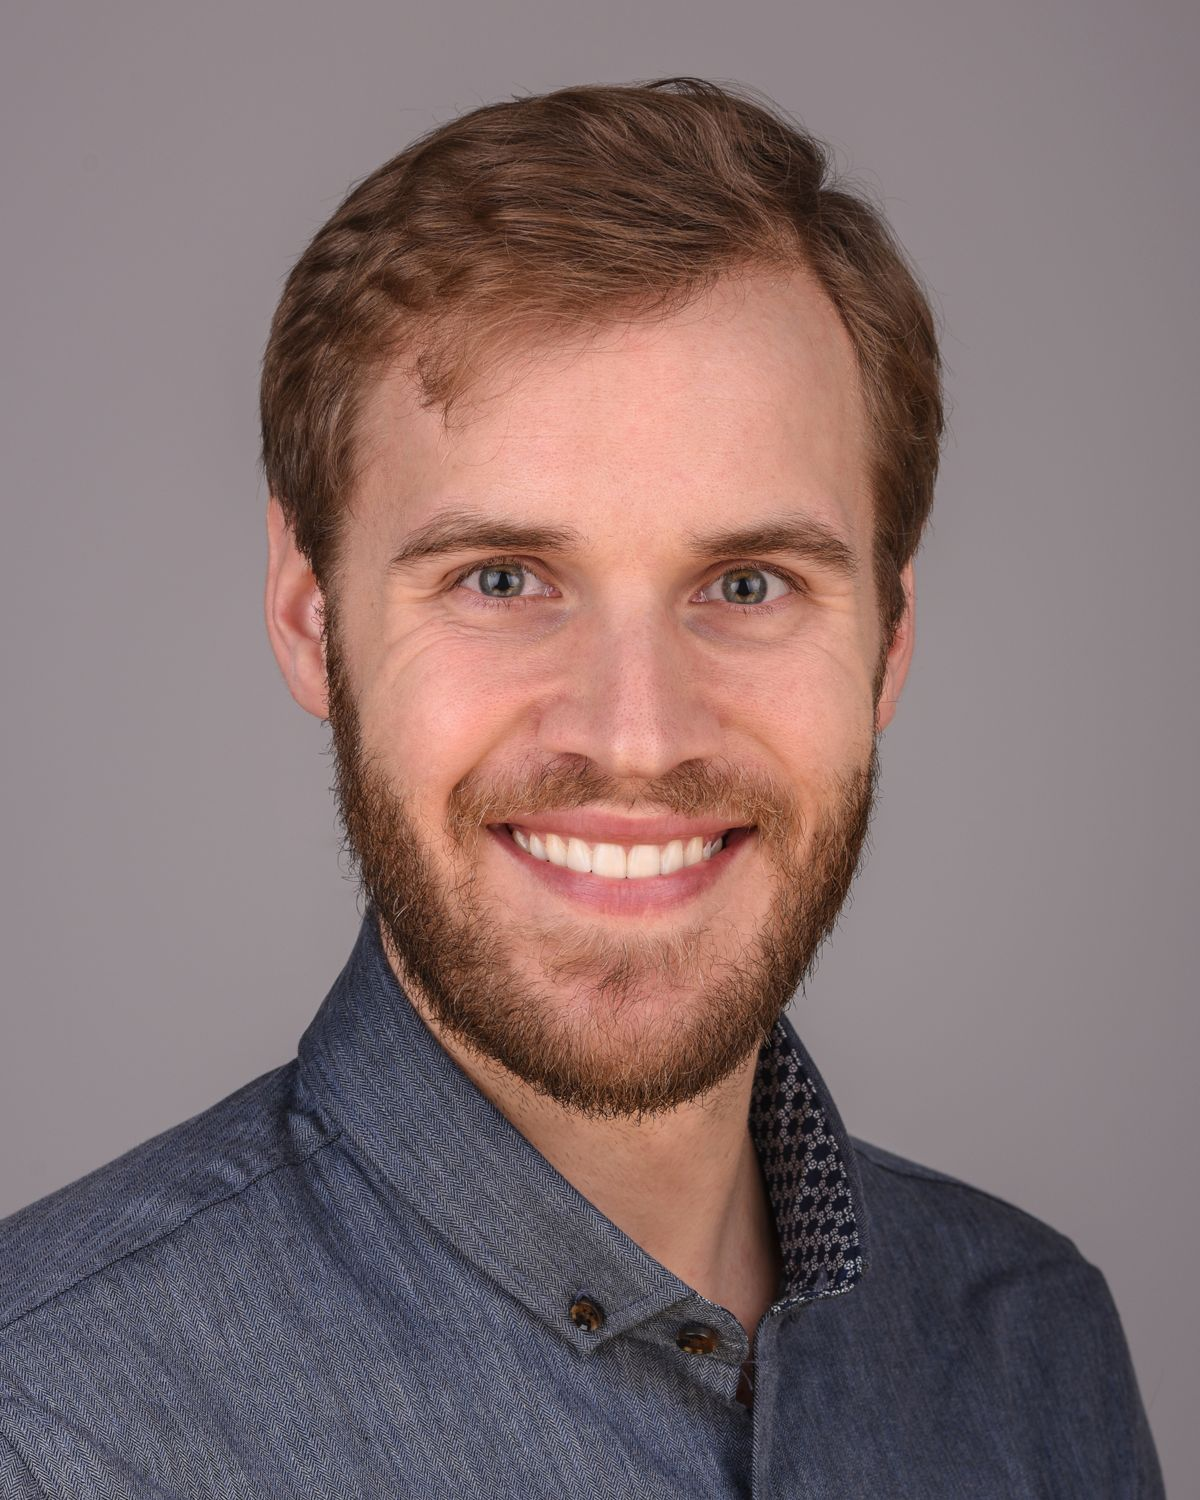
\includegraphics[width=0.25\linewidth]{colin.jpg}
\end{figure}

\begin{CJK}{UTF8}{ipxma}
\begin{center}
  フルスタック開発者・オープンソース経験者 \\
  カナダの「生産的開発者ランキング」トップ20に選抜 \\
\end{center}

%--------PROGRAMMING SKILLS------------
\section{能力}
\resumeSubHeadingListStart
\item{\textbf{プログラミング言語}: Haskell, Rust, Go, Scala, Python, C}
\item{\textbf{ウェブ技術}: Terraform, GraphQL, AWS, Docker, Web Assembly}
\item{\textbf{その他}: Linux, Git, SQL, MongoDB, Apache Spark}
  \resumeSubHeadingListEnd


  %-------------------------------------------

%-----------EXPERIENCE-----------------
\section{経歴}
  \resumeSubHeadingListStart

    \resumeSubheading
      {Kadena}{アメリカ・ニューヨーク}
      {Haskell 開発者}{2018年8月から2020年5月まで}
      \resumeItemListStart
        \resumeItem{バックエンド開発}
                   {Core developer of the Kadena Public Blockchain (Chainweb). Designed and implemented its Difficulty Adjustment algorithm. Pioneered Chainweb's mining algorithm and wrote its client, chainweb-miner.}

         \resumeItem{システム管理}
                    {Worked as the main system administrator for Kadena web servers. Managed servers on AWS with Terraform and NixOS.}
         \resumeItem{ドキュメンテーション}
                    {Wrote extensive documentation in both Japanese and English.}
         \resumeItem{会社代表}
                    {Represented the company as a speaker at conferences in Japan, the USA, and Canada.}
      \resumeItemListEnd

    \resumeSubheading
        {Azavea}{アメリカ・フィラデルフィア}
        {Scala 開発}{2016年5月から2017年12月まで}
        \resumeItemListStart
          \resumeItem{GeoTrellis}{Open-source developer on the GeoTrellis project, a library suite for batch processing of geographic data using Apache Spark. Researched, designed, and implemented GIS algorithms.}
          \resumeItem{VectorPipe}{Wrote a library to process Vector Tile data through GeoTrellis.}
          %% \resumeItem{VectorTiles}{Wrote Haskell and Scala libraries that implement the Mapbox Vector Tiles spec.}
          \resumeItem{システム管理}{Used Docker and Terraform extensively to manage production systems on AWS.}
        \resumeItemListEnd

    \resumeSubheading
        {Adenda Media}{カナダ・バンクーバー}
        {Scala 開発}{2014年5月から2016年4月まで}
        \resumeItemListStart
          \resumeItem{バックエンド開発}{Maintained and enhanced a Play + MySQL backend.}
          \resumeItem{フロントエンド開発}{Extended a Twitter Bootstrap-based web application.}
          \resumeItem{人工知能}{Implemented a content recommendation system using Apache Spark's MLlib.}
        \resumeItemListEnd

    \resumeSubheading
        {佐世保市教育委員会}{長崎県佐世保市}
        {英語準教師 (ALT)}{2010年8月から2013年7月まで}
        \resumeItemListStart
          \resumeItem{小中学校の英語教育}{Taught English to over a thousand Middle School students. Created lesson plans, supported Japanese colleagues, and helped grade tests.}
          \resumeItem{英語部担当}{Ran an English Club for students who wanted extra practice. Trained studets to participate in English speech contests.}
        \resumeItemListEnd


  \resumeSubHeadingListEnd



%-----------EDUCATION-----------------
\section{学歴}
\resumeSubHeadingListStart
\resumeSubheading
{サイモンフレーザー大学}{カナダ・バンクーバー}
{Computing Scienceの学士号}{2013年9月から2016年4月まで}
\resumeSubheading
{佐賀大学}{佐賀県佐賀市}
{SPACEプログラム短期留学}{2008年9月から2009年8月まで}
\resumeSubheading
{マニトバ大学}{カナダ・ウィニペグ}
{四年間の学士号}{2006年9月から2010年4月まで}
\resumeSubHeadingListEnd

%-----------CERTIFICATIONS-----------
\section{資格・免許}
\resumeSubHeadingListStart
\resumeSubItem{日本語能力試験 (JLPT)}{N1}
\resumeSubItem{漢字検定}{準二級}
\resumeSubHeadingListEnd

%-----------PROJECTS-----------------
\section{オープンソース}

主なプロジェクト:

\resumeSubHeadingListStart
\resumeSubItem{\href{https://github.com/aurapm/aura}{Aura}}{(Haskell) Arch Linuxのパッケージ管理ツール。数千人のユーザーを誇る。}
\resumeSubItem{\href{https://github.com/fosskers/active}{Active}}{(Go) Github Actionsを更新するツール。}
\resumeSubItem{\href{https://github.com/fosskers/credit}{Credit}}{(Rust) プロジェクト活躍を測るツール。}
\resumeSubItem{\href{https://github.com/fosskers/mapalgebra}{MapAlgebra}}{(Haskell) 地理情報システムのライブラリ。}
\resumeSubItem{\href{https://github.com/fosskers/rs-kanji}{Kanji}}{(Rust) 日本漢字の分析。}
\resumeSubHeadingListEnd

%-----------HOBBIES-----------
\section{趣味}
\resumeSubHeadingListStart
\resumeSubItem{オープンソース開発}{Aura・ライブラリの実装や保守}
\resumeSubItem{クライミング}{トップロープ・ボルダリング・大会にも参加}
\resumeSubItem{言語学習}{日本語・ドイツ語・イタリア語・エスペラント語}
\resumeSubHeadingListEnd

%
\end{CJK}
\end{document}
